
\chapter{Methods} % Main chapter title

\label{Chapter3} % For referencing the chapter elsewhere, use \ref{Chapter1} 

%----------------------------------------------------------------------------------------

% Define some commands to keep the formatting separated from the content 


\section{Generate external Module Map of T cell expression patterns}

\subsection{Introduction to reference dataset- ImmGen}

ImmGen is a consortium whose main aim is to establish a comprehensive resource of the gene networks operating in the mouse hematopoietic system. The 2012 release is comprised of 816 microarray expression profiles from 246 mouse immune cell types ~\autocite{Joj2013,Sha2013}. The cell types included in this dataset span all major hematopoietic lineages, namely: stem and progenitor cells, granulocytes, monocytes, macrophages, dendritic cells (DC), natural killer (NK) cells, B cells, and T cells ($\alpha\beta$ cells, Tregs, $\gamma\delta$ cells and natural killer CTLs) ~\autocite{Joj2013}. A given cell type was usually sampled from multiple tissues which should result in more in-depth and reliable profiling. As highlighted in Figure 3.1 researchers observed in most cases that the closer two cell populations are in terms of lineage, the more their expression profiles are correlated. 

\begin{figure}[H] 
    \centering
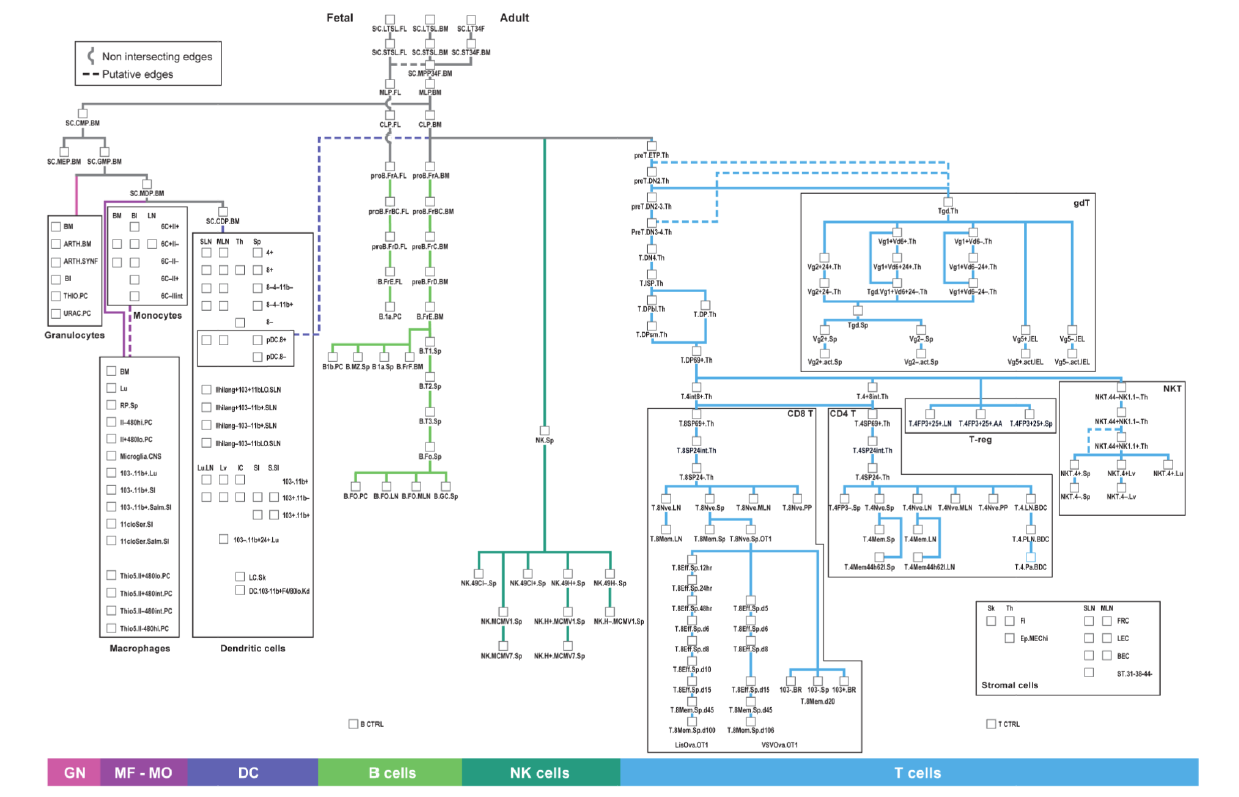
\includegraphics[width=0.9\textwidth]{Figures/Chapter3/immgen_lineage_tree.png}
\caption{\small{Lineage tree of the hematopoietic mouse cell types profiled by the Immunological Genome consortium ~\autocite{Joj2013}} }
    \label{fig:7}
\end{figure}

\subsubsection{Published ImmGen modules}

The ImmGen consortium has published modules of co-expressed genes which are organised into two levels of clustering, namely coarse and fine-grained ~\autocite{Joj2013}. In brief, 81 coarse-grained modules were initially defined using the hierarchical clustering method known as Super Paramagnetic Clustering (SPC) ~\autocite{Bla1996}. The SPC technique is based on the physical properties of an inhomogeneous ferromagnetic model and does not require input of a pre-defined value for the number of clusters between which the data must be split. Instead the algorithm assigns a Potts spin to each data point and attempts to identify the number that best fits the inherent structure of the dataset itself ~\autocite{Bla1996}. When run with default parameters SPC produced 80 stable clusters which were called coarse-grained modules C1-C80. Coarse module C81 contains the remaining unclustered genes and hence can be thought of as a "bin" module ~\autocite{Joj2013}. 

Subsequently, each coarse-grained module was partitioned to fine-grained modules. SPC could not further refine the coarse-grained modules and so affinity propagation clustering was employed ~\autocite{Fre2007}, using correlation as the affinity measure. Although not all genes could be included in this analysis, clustering resulted in 334 fine-grained modules, referred to in the text as fine modules F1-F334. On average each coarse-grained module contained 3.9 fine-grained modules ~\autocite{Joj2013}. 

The focus of this project is primarily centred around the transcriptional profiles of T cells alone and the ImmGen module database naturally seemed a good potential source of such T cell specific gene modules. Interestingly however, despite the plethora of data incorporated into the ImmGen analysis, only one course module, C18 (entitled "T-cell activation: TCR/CD3 complex genes, their downstream regulation"), appears to be specifically up-regulated in T cell subtypes (see Figure 3.2). This module contains 146 genes and was subdivided into 5 fine-grained modules (F90 - F94). 

\begin{figure}[H] 
    \centering
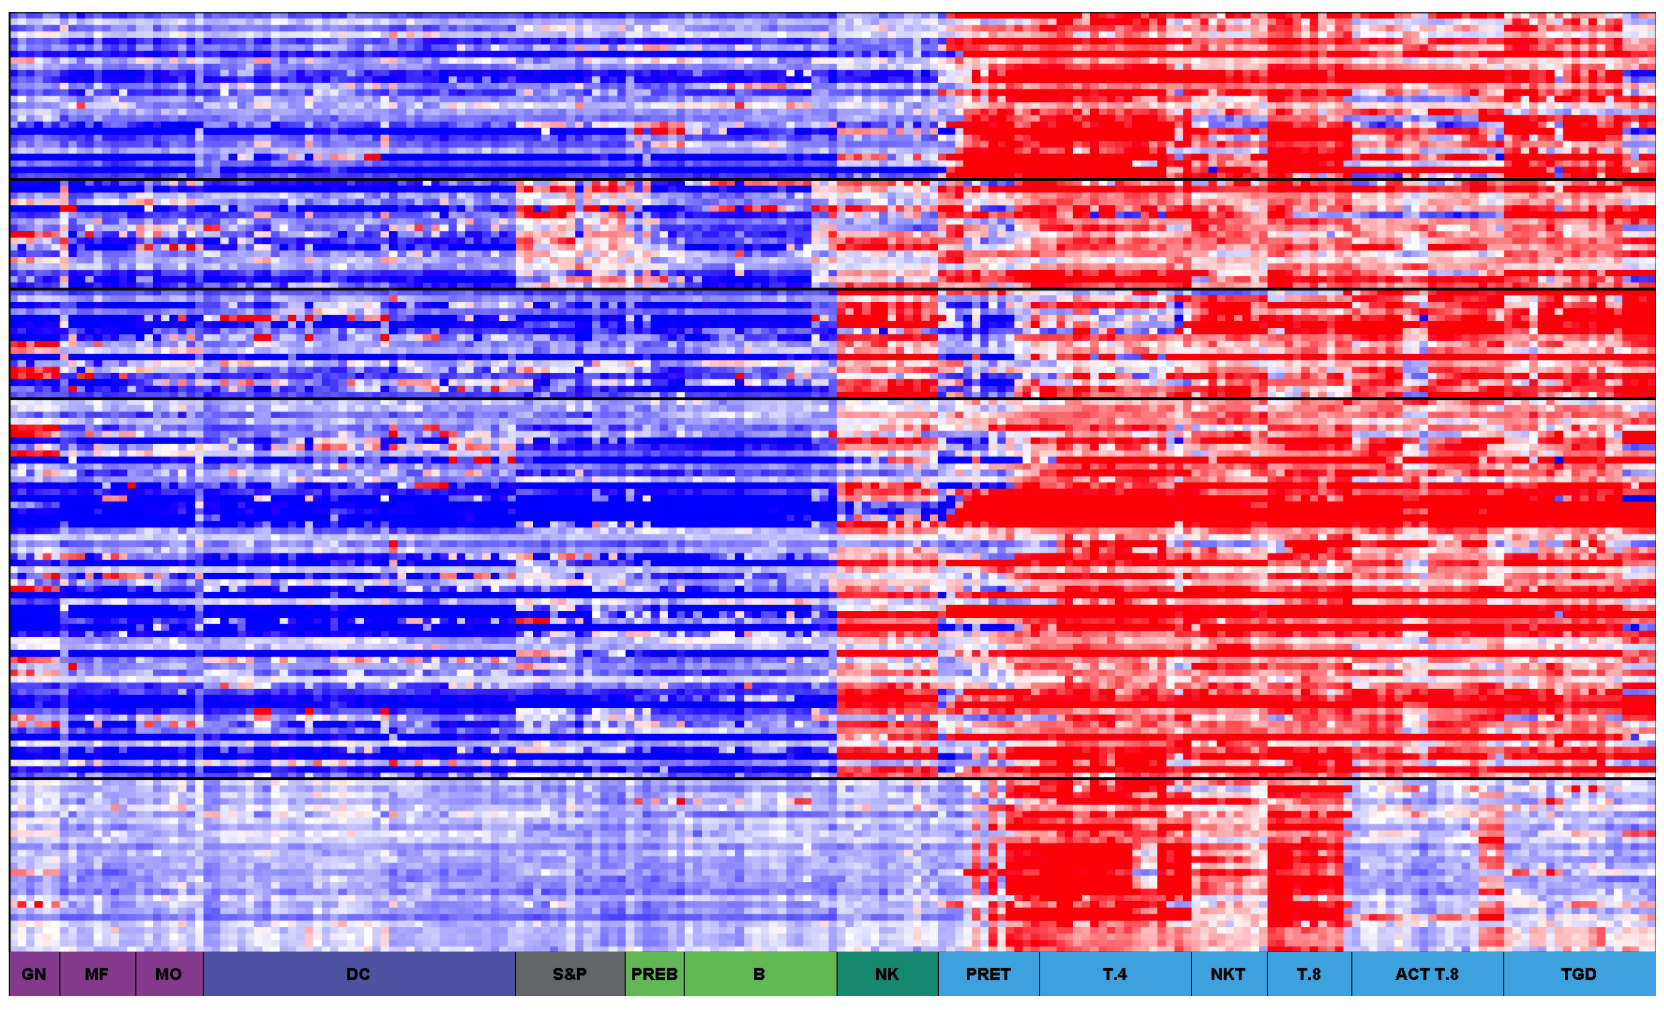
\includegraphics[width=0.7\textwidth]{Figures/Chapter3/C18_t_cell_activation.png}
\caption{\small{The mean centred expression of module C18 genes (rows) in each population of cells (column). Red denotes high expression levels, blue low expression levels. Major lineages are given at the bottom. Adapted from  ~\autocite{ImmGen}} }
    \label{fig:8}
\end{figure}

We therefore wondered whether by utilising the publicly available expression data from the ImmGen resource and extracting only those samples originating from T cell populations, we could re-cluster the genes in a manner that could generate a "Module Map" of T cell specific expression patterns. The following sections briefly summarise the data extracted for re-clustering as well as the various methods employed for the generation of gene modules. 

\subsubsection{T cell Dataset}

The microarray expression data used for gene clustering represents a subset of the complete ImmGen dataset ~\autocite{Joj2013}. Only T cell samples were included, resulting in an input data matrix consisting of 21755 gene expression values sampled across 89 samples. As outlined above, this T cell only dataset contained samples from $\alpha\beta$ cells, Tregs, $\gamma\delta$ cells and natural killer CTL populations. 

\subsection{Overview of clustering techniques employed}

\subsubsection{\underline{Weighted Gene Correlation Network Analysis (WGCNA)}}

In Chapter \ref{Chapter1} we briefly discussed the use of correlation matrices in the analysis of large datasets. Langfelder and Horvath built on this methodology to develop an R package to cluster highly correlated genes and analysing the functional properties of the resulting modules ~\autocite{Lan2008}. The WGCNA package they developed contains a comprehensive set of functions for performing a correlation network analysis of large, high-dimensional data sets. Functions available in the WGCNA package can be divided into several categories which also summarise the stages of a typical workflow when using this package to identify modules of genes within a microarray dataset. These categories are:

\begin{enumerate}
    \item Network Construction 
    \item Module Detection 
    \item Module and Gene Selection 
    \item Calculations of Topological Properties 
    \item Visualisation
    \item Interfacing with External Software 
\end{enumerate}

The following provides a brief overview of these analytical steps. 

\myparagraph{Network Construction}

In order to fully describe a gene network, it is necessary to calculate it's adjacency matrix which is a symmetric \textit{n} x \textit{n} matrix with entries in [0, 1] whose component \textit{$a_{ij}$} encodes the network connection strength between nodes \textit{i} and \textit{j}.. Computation of this matrix however requires that we first define the co-expression similarity \textit{$s_{ij}$} which is typically defined as the absolute value of the unsigned correlation coefficient between the profiles of nodes \textit{i} and \textit{j} as follows: 

\begin{equation}
    s_{ij}^{unsigned} = |cor(x_i, x_j)|
\end{equation}

One notable downside of taking the absolute value of the correlation is that biological information regarding whether genes are activated or repressed is usually lost. It is however possible to transform the similarity matrix defined in equation 3.1 in order to take account of the sign of the correlation between genes expression profiles: 

\begin{equation}
    s_{ij}^{signed} = 0.5 + 0.5cor(x_i, x_j)
\end{equation}

In the case of both $s_{ij}^{unsigned}$ and $s_{ij}^{signed}$, the similarity takes on a value between 0 and 1 but for two genes with opposing directions of expression profiles the unsigned similarity measure will equal 1, whereas it will be 0 if the signed measure is applied. \\

Given the similarity matrix as defined in equation 3.1 and 3.2, the corresponding adjacency matrix \textit{$a_{ij}$} is quantified by thresholding the chosen similarity matrix. 'Hard' thresholding (dichotomizing) the similarity measure $S = [s_{ij}]$ results in an unweighted gene co-expression network. Specifically an unweighted network adjacency is defined according to:

\begin{equation}
    a_{ij} = \bigg\{\frac{1 \text{ if } s_{ij} \geq \tau;}{0 \text{ otherwise}}
\end{equation}

where $\tau$ represents the "hard" thresholding parameter. Two genes are said to be linked i.e. \textit{$a_{ij}$} =1, when the absolute correlation between their expression profiles is greater than $\tau$. As the relationship between any two genes is classified in a binary manner, using a "hard" threshold can result in the loss of potentially biologically relevant information. However, WGCNA allows the user to instead apply a "soft" threshold which enables the continuous nature of the co-expression to be preserved by calculating a weighted network adjacency. This is achieved by raising the co-expression similarity to a power: 

\begin{equation}
    a_{ij} = s_{ij}^{\beta}
\end{equation}

$\beta \geq 1$ must apply for equation 3.4 to correctly calculate the adjacency. 

The calculation of adjacency matrices for both weighted and unweighted networks require the user to choose threshold parameters and one way this can be achieved within the WGCNA package environment is by applying the approximate scale-free topology criterion ~\autocite{Zha2005}.

\myparagraph{Module Detection}

One of the primary functions of the WGCNA package is to identify modules which are defined as clusters of densely interconnected genes. By default, the topological overlap measure (TOM) is used to calculate the network interconnectedness ~\autocite{Zha2005}. A key feature of WGCNA is that it does not require input of  \textit{a priori} defined gene sets, but instead identifies gene modules using unsupervised clustering. Hierarchical clustering using the standard R function hclust (described in a later section) is the default method. The blockwiseModules function facilitates network construction and module detection in large data sets by pre-clustering nodes into large clusters, or blocks, using a variant of k-means clustering. Hierarchical clustering is subsequently applied to each block in turn and gene modules are defined as branches of the resulting dendrogram. Lastly, modules wit highly correlated eigengenes are merged. 

Once modules have been detected, it is possible to summarise the expression profiles of genes within a given module using a variety of features. One option is to use the moduleEigengenes function which represents the expression profiles of genes within the \textit{q}-th module as \textit{$E^(q)$}, the first principal component of the expression matrix. The eigengene \textit{E} is equivalent to a weighted average expression profile.

\myparagraph{Module and Gene Selection}

The WGCNA package also contains functions to assist in identifying genes and modules that are likely to be biologically significant in a particular setting. In general terms, a gene significance measure is defined as a function \textit{GS} that assigns a non-negative number to each gene, \textit{i}. The higher \textit{GS\textsubscript{i}} the more biologically significant the gene. The interpretation of \textit{GS} measures will vary depending on the experimental context, but a high value could for example indicate pathway membership. Additionally, a microarray sample trait T can be used to define a trait-based gene significance measure as the absolute correlation between the trait and the expression profiles, i.e.:

\begin{equation}
    GS_{i} = |cor(x_i, T)|
\end{equation}


A measure of module significance can be calculated as the average gene significance, \textit{GS}, across the module genes (Figure 3A). Furthermore, when incorporating information relating to a sample trait \textit{T}, a measure of statistical significance between the module eigengene \textit{E} and the trait \textit{T} can be defined.

\myparagraph{Calculation of Topological Properties}

The WGCNA package implements several functions, including softConnectivity, intramodularConnectivity, TOMSimilarity, clusterCoef, and networkConcepts for computing gene network topological properties, many of which we defined in Chapter \ref{Chapter1}.

\myparagraph{Visualisation}

Both modular structure and network connections can be visualised in multiple ways within the WGCNA environment. To give an example, the co-expression module structure can be visualised by heatmap plots of gene-gene connectivity using the function TOMplot or as a multi-dimensional scaling plot. Relationships among modules can also be summarised by a hierarchical clustering dendrogram of their eigengenes, or a heatmap plot of the corresponding eigengene network. 

\myparagraph{Interfacing with External Software}

Once analysis of a dataset is complete, the WGCNA package contains a number of features to aid in integration of results with other network visualisation packages as well as gene ontology analysis software. For example, the R functions exportNetworkToVisANT and exportNetworkToCytoscape allow the export of networks in a format compatible with VisANT ~\autocite{Hu2008} and Cytoscape ~\autocite{Sha2003}, respectively. Gene lists compatible with Gene Ontology packages e.g. David ~\autocite{Den2003} are also easily generated. 

\subsubsection{\underline{Agglomerative Hierarchical clustering (Hclust)}}

Hierarchical clustering (also referred to as hierarchical cluster analysis) is a method of cluster analysis which seeks to build a hierarchy of clusters. The algorithm proceeds in a bottom-up manner whereby each object, in this instance gene, is initially considered as a single-element cluster (leaf). With each consecutive iteration, the two clusters that are the most similar are combined into a new bigger cluster (nodes). This procedure is repeated until all points are member of just one single big cluster (root). The result is a tree-based representation of the observations which is called a dendrogram. Hierarchical clustering in R was performed using the \textit{hclust()} function of the "cluster" package. 

\myparagraph{Determining Cluster Dissimilarity}

In order to decide which clusters should be combined a measure of dissimilarity between sets of observations is required. In most methods of hierarchical clustering, this is achieved by use of an appropriate measure of distance between pairs of observations (the metric), and a linkage criterion which specifies the dissimilarity of groups/clusters as a function of the pairwise distances of observations within them.

\underline{Metric}

The choice of an appropriate metric will influence the shape of the clusters, as some elements may be close to one another according to one distance and farther away according to another. For example, in a 2-dimensional space, the distance between the point (1,0) and the origin (0,0) is always 1 according to the usual norms, but the distance between the point (1,1) and the origin (0,0) can be 2 under Manhattan distance, $\sqrt{2}$ under Euclidean distance, or 1 under maximum distance.

\underline{Linkage Criteria}

The linkage criterion determines the distance between sets of observations as a function of the pairwise distances between observations. There are a number of different methods available to compute these distances, the most popular being: 

\begin{itemize}
    \item Maximum or complete linkage clustering: It computes all pairwise dissimilarities between the elements in cluster 1 and the elements in cluster 2, and considers the largest value (i.e., maximum value) of these dissimilarities as the distance between the two clusters. It tends to produce more compact clusters.
    \item Minimum or single linkage clustering: It computes all pairwise dissimilarities between the elements in cluster 1 and the elements in cluster 2, and considers the smallest of these dissimilarities as a linkage criterion. It tends to produce long, “loose” clusters.
    \item Mean or average linkage clustering: It computes all pairwise dissimilarities between the elements in cluster 1 and the elements in cluster 2, and considers the average of these dissimilarities as the distance between the two clusters. 
    \item Centroid linkage clustering: It computes the dissimilarity between the centroid for cluster 1 (a mean vector of length p variables) and the centroid for cluster 2.
    \item Ward’s minimum variance method: It minimizes the total within-cluster variance. At each step the pair of clusters with minimum between-cluster distance are merged.
\end{itemize}

\myparagraph{Hierarchical clustering and correlation based distance}

Typical statistical programming functions for hierarchical clustering use Euclidean distance measures as default metric. However, it is also possible to use correlation-based distance measures which are often more suited to the clustering of gene expression data. In such analyses, a pairwise correlation matrix between items is computed using the function \textit{cor()} which can calculate either “pearson”, “spearman” or “kendall” correlation method. Next, the correlation matrix is converted as a distance matrix and finally clustering can be computed on the resulting distance matrix.

Correlation-based distance considers two observations to be similar if their features are highly correlated, even though the observations themselves may lie far apart in terms of Euclidean distance.

It is important to note that, when the data are standardised, there exists a functional relationship between the Pearson correlation coefficient and the Euclidean distance:

\begin{equation}
d_{euc}(x,y) = \sqrt{2m[1-r(x,y)]}
\end{equation}
Where \textit{x} and \textit{y} are two standardised \textit{m}-vectors with zero mean and unit length.

\subsubsection{\underline{K-means}}

\myparagraph{Overview}

K-means clustering is an unsupervised learning algorithm, which iteratively assigns each data point to one of \textit{K} groups based on the features that are provided. Data points are clustered based on feature similarity. The results of the K-means clustering algorithm are as follows:

\begin{enumerate}
    \item The centroids of the K clusters, which can be used to label new data
    \item Labels for the training data (each data point is assigned to a single cluster)
\end{enumerate}

Each of the cluster centroids will possess a feature weight which can be used to qualitatively interpret what kind of group each cluster represents.  

\myparagraph{Algorithm}

The main idea of \textit{k}-means clustering, where Euclidean distance is used as a metric and variance is used as a measure of cluster scatter, is to define \textit{k} centroids, one for each cluster. The positioning of these centroids is a crucial variable as different locations will produce different results. The ideal is therefore for the centroids to be placed as far from one another as possible. Once initial positions have been fixed, the next step is to take each point belonging to the dataset and associate it to the nearest centroid. When all points have been assigned, the first step is completed and an early clustering has been completed. At this point it is necessary to re-calculate \textit{k} new centroids as barycenters of the clusters resulting from the previous step. After we have these \textit{k} new centroids, new assignments must be made between the same data set points and the nearest new centroid. A loop is thus generated within which the \textit{k} centroids change their location step by step until stable clusters have formed. 

\myparagraph{Choosing \textit{K}}

The algorithm described above finds the clusters and data set labels for a particular pre-chosen \textit{k}. To find the number of clusters in the data, the user must run the \textit{k}-means clustering algorithm for a range of values of \textit{k }and compare the results. In general, there is no perfect method for determining exact value of \textit{k}, but an accurate estimate can be obtained using a number of techniques.

One of the metrics that is commonly used to compare clustering results across different values of \textit{k} is the mean distance between data points and their cluster centroid. Since increasing the number of clusters will always reduce the distance to data points, increasing \textit{k} will always decrease this metric, to the extreme of reaching zero when \textit{k} is the same as the number of data points. Thus, the mean distance to the centroid as a function of \textit{k} is plotted and the "elbow point," where the rate of decrease sharply shifts, can be used to approximately determine the value of \textit{k} which best fits the data. It is important to note however that an inappropriate choice of \textit{k} may lead to poor results. 

\newpage

\section{Analysis of current/in-house GvHD (MataHari and B6) data}

\subsection{Differential gene expression (DE) analysis}

\subsubsection{Background}

Often when conducting microarray based experiments we are seeking to quantify which genes undergo changes in expression levels between sample groups. This methodology allows us to swiftly identify up- and down-regulated collections of genes in a given condition (either biological or experimental it nature). Each sample obtained from a microarray study will consist of a number of replicates and these will typically be summarised as the mean of the replicate expression levels. Thus in differential expression analysis, we are comparing mean differences in mRNA transcript production between the samples in question. 

\subsubsection{Statistical tests}

There are multiple approaches to statistically quantify whether expression level differences between samples are significant and each has it's own benefits and drawbacks. Almost all are focused on so called "two-class" problems and are only appropriate where the number of probes (\textit{p}) is much greater than the number of samples (\textit{n}). The method employed for establishing differentially expressed gene lists in this study is an empirical Bayes moderated t-statistic and it is this approach, together with the standard t-statistic upon which it is based, that will be covered here. 

\subsubsection{The t-statistic}

The basic formula for calculating a t-test for independent samples is:

\begin{equation}
t_g = \frac{\bar{X}_1 - \bar{X}_2} {\sqrt{\frac{\sigma^2_1}{N_1}\frac{\sigma^2_2}{N_2}}} \label{t-statistic}
\end{equation}

where $\bar{X}_i$ and $\sigma_i$ are the mean and variance of sample \textit{i} respectively. \\
\\
Whether the null hypothesis should be rejected is determined by comparing the value of $t_g$ obtained using the above calculation to the critical value. This critical value is defined as: 

\begin{equation}
t_{\alpha/2,n–p-1,}
\end{equation}

where $\alpha$ is the significance level, \textit{n} is the number of observations in the  sample, and \textit{p} is the number of variables.

If the absolute value of $t_g$ is greater than the critical value, the null hypothesis should be rejected in favour of the alternative. 

\myparagraph{Null hypothesis}

The null hypothesis of the t-test is that there is no statistically significant difference between the means of the two samples being compared i.e. 

\begin{equation}
H_o: \bar{X}_1 = \bar{X}_2 \label{t-statistic}
\end{equation}

\myparagraph{Assumptions}

The assumptions of the t-test are: 

\begin{enumerate}
    \item \textbf{Normally distributed data} - The populations from which the samples have been drawn should follow the normal distribution. 
    \item \textbf{Independence} - As is the case for all statistical tests of this nature, individual observations are assumed to be independent of one another.
    \item \textbf{Equal standard deviations} - The standard deviation of the populations should be equal.
\end{enumerate}

\myparagraph{Limitations}

The t-test has several limitations. Firstly, the variance in small samples can often be relatively "noisy" and this may have a substantial negative impact on the reliability of results. Secondly, while genes with small fold-change might be significant from a  statistical perspective, they may not be of interest biologically. 


\myparagraph{Computation in R} 

No computations of the t-test statistic were performed in this work with an adapted version, namely the empirical Bayes moderated t-statistic being preferred. 

\subsection{Fisher's Exact test}

\subsubsection{Background}

The Fisher's Exact Test of independence is a statistical tool used in cases where two nominal variables are measured and one wishes to assess whether the occurrence of of one of the variables is dependent upon the value of the other. The main application of this methodology is in situations where data exists in categorical format resulting from two-way classification of observations and so can be written in the form of a $2 \times 2$ contingency table. Thus this analysis represents a test of association between the two categories. Fisher's Exact Test is appropriate for analysis of small datasets and in this context is more accurate than the chi-squared or G-test methods. 

In this work we sought to quantify whether the observed number of differentially expressed genes assigned to a given module (X) was higher than that expected by chance. 

\subsubsection{Null hypothesis}

The null hypothesis of the Fisher's Exact Test is that the relative proportions of one variable are independent of the second variable, i.e. the proportions at one variable are the same for different values of the second variable. 

\subsubsection{Calculation of test statistic}

Consider the following generalised $2 \times 2$ contingency table:

\begin{center}
\begin{tabular}{ |c|c|c|c| } 
 \hline
  & \textbf{Not in module X} & \textbf{In module X} & Row Total \\ 
 \hline
 \textbf{Non DE} & a & b & \textit{a $+$ b} \\
 \hline
 \textbf{DE} & c & d & \textit{c $+$ d} \\
 \hline
Column Total & \textit{a $+$ c} & \textit{b $+$ d} & \textit{a $+$ b $+$ c $+$ d ($=$n)}\\
\hline
\end{tabular}
\end{center}

Given this notation, Fisher showed that the probability of obtaining any such set of values could be established using the hypergeometric distribution as follows:

\begin{equation}
p = \frac{\binom{a+b}{a} \binom{c+d}{c}} {\binom{n}{a+c}} = \frac{(a+b)!(c+d)!(a+c)!(b+d)!}{a!\, b!\, c!\, d!\, n!} \label{hypergeo}
\end{equation}

When substituted with actual data, equation \eqref{hypergeo} gives the exact hypergeometric probability of obtaining the observed arrangement of the data, assuming the marginal totals (i.e., assuming the row and column totals shown in the margins of the table are given), under the null hypothesis that genes are all equally likely to be differentially expressed whether they form part of module X or not.  

Although application of the above formula facilities calculation of the exact probability of any arrangement of the \textit{n} observations into the four table cells, Fisher proved that in order to generate a significance level for the test result it is only necessary to do so for cases where two linked conditions are met. These are:

\begin{enumerate}
    \item  The marginal totals are the same as in the observed table;
    \item and among those, only where the arrangement is as, or more extreme than the observed arrangement
\end{enumerate}

Having computed these additional probabilities, the significance of the observed data can be obtained by summation of these values together with that calculated using the actual frequencies. This is a one-tailed test however which, in practice, is rarely suitable. It is virtually always necessary to conduct a two-tailed test, which in addition to the calculations outlined above, requires the inclusion of tables with combinations as equally extreme as the observed but in the opposite direction. This is something of a challenge as there is no clear cut threshold for what values should qualify as "extreme". There are multiple approaches to address this issue, the most common of which is to sum the probabilities of all combinations possessing probabilities lower than, or equal to, that of the observed data. 

\subsubsection{Assumptions}

Fisher's Exact Test carries two main assumptions, namely: 

\begin{enumerate}
    \item \textbf{Independence} - Samples are assumed to be independent of one another. The same should be true of the variables used for classification. 
    \item \textbf{Fixed totals} - Although often not adhered to in biological studies, this test is only actually exact when both the row and column totals are fixed or "conditioned". 
\end{enumerate}

\subsubsection{Limitations}

Whilst the Fisher's Exact Test may seem well suited for assisting in our search for potential enrichment of differentially expressed genes within module lists, we believe there is one potentially key feature that it is lacking. This statistical test does not take any account of the relative direction or size of the change in expression for differentially expressed genes within a given module. We believed that incorporating this aspect of the dataset could potentially add significant power to our analyses, as well as offering the opportunity to uncover more biologically relevant associations. 

\subsubsection{Computation in R} 

All computations of the Fisher's Exact Test statistic were performed in R using the fisher.test() function of the \textit{stats} package. 

\subsection{Module-based differential expression analysis - New refined testing protocol}

\subsubsection{Background}

In order to quantify potentially significant associations of gene modules (specifically those derived from WGCNA or similar algorithms) between tissue types and/or between conditions, we developed a gene based association test that, unlike aforementioned statistical tests of association, incorporates information regarding the magnitude and sign of the differential expression effect size observed for each gene.

\subsubsection{Calculation of test statistic}

Given that the purpose of this test is to assess whether genes are consistently over-expressed in a set of cases compared to controls, the initial step is to transform a gene's \textit{p}-value into a chi-squared statistic $X_\textit{i}$ with one degree of freedom, at which point the \textit{T} statistic can be calculated by summing, for all genes, the $X_\textit{i}$, if $X_\textit{i}$ is positive, or 0, if it is negative. Under the null, the distribution of this $X_i$ is determined by applying the assumption that for any given gene, the chance of under- or over-expression is 50\%. An important feature of this testing protocol is that, if it is known that this assumption does not hold for a particular dataset, this parameter can be refined by computing the genome-wide probability of over-expressed genes. Whatever the genome-wide proportion of over-expressed genes, the corresponding probability of observing \textit{K} over-expressed genes among the \textit{n} genes that form a module can be computed using a binomial distribution. As any given \textit{K} represents the sum of \textit{K} one degree of freedom chi-square distributions, the statistic \textit{T} is chi-squared with \textit{K} degrees of freedom. The probability of observing a test statistic greater than the observed value \textit{T} can then be computed using a weighted sum of probabilities, summing over all possible values of \textit{K}. 

Whilst the above explanation is based upon the proportion of over-expressed genes, the calculations are equivalent if all genes are predicted to be under-expressed. If a mixture of over- and under-expressed genes is expected, the \textit{T} statistic is then summed over all genes in an appropriate manner to reflect the said combination.

\subsubsection{Data simulations}

Having developed the module-based refined testing protocol for differential expression datasets, we analysed its behaviour and performance on simulated gene module data. To this end we generated two simulated datasets, one to assess how our module-based test handles data matching the null, where the gene-based "direction of effect" within a module is not relevant and a second, alternative, dataset where a proportion of genes within a module exhibit a skewed direction in terms of the sign ($+/-$) of the log(fold change) in expression levels between artificially simulated "conditions". The next two sections provide details of the simulated datasets (16000 "genes") used to test the performance of our module-based test as well as a summary of the observed findings. 

\myparagraph{Simulating under the null}

We expect that when supplied with data consisting of uniformly distributed \textit{p}-values and direction (i.e. genes have a 50-50 chance of going up/down), our \textit{T} statistic should behave as a chi-squared with two degrees of freedom. To determine whether this predicted distribution of \textit{p}-values was observed, we generated a dataset of 16000 data points, each with a \textit{p}-value and assigned direction drawn from uniformly distributed populations (min = 0, max = 1 for \textit{p}-values, min = -1, max = 1 to acquire direction sign). "Modules", each containing 200 simulated gene data points were sampled, put through the refined testing analysis and the resulting distribution of test statistic \textit{p}-values plotted against the corresponding expected order statistics (using the \textit{qq.chisq} function of the \textit{snpMatrix} R package). This plot is shown in Figure 3.3 below. 

\begin{figure}[H] 
    \centering
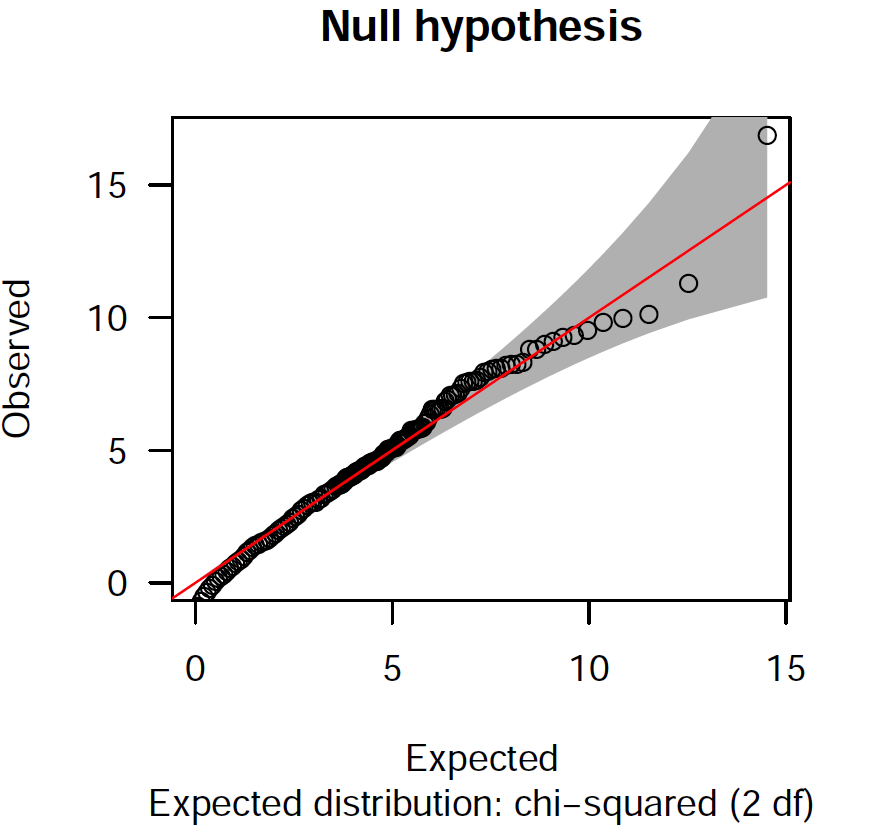
\includegraphics[width=0.5\textwidth]{Figures/Chapter3/simulated_null_skewedDir.png}
\caption{\small{Distribution of module-based refined test statistic \textit{p}-values simulated under the null plotted against the corresponding expected order chi-squared statistics (two degrees of freedom)} }
    \label{fig:9}
\end{figure}

It is evident from the above plot that, when provided with uniformly distributed data (the null situation), the \textit{T} statistics generated by our test are indeed a good fit to a chi-squared with two degrees of freedom. This is an encouraging and reassuring result as it indicates that our analysis is not falsely amplifying, or worse still manufacturing, significant \textit{p}-values when none are present in the test dataset. 

\myparagraph{Simulating under the alternative}

To establish how our module-based test performed on data fitting the alternative hypothesis where the direction of effect is skewed for the portion of genes that are significantly up-regulated/over-expressed, we created a simulated dataset similar to that used to evaluate our statistic under the null, but this time while the \textit{p}-values remained uniformly distributed the proportion of up-regulated genes varied (see Figure 9). Again, 16000 data points were generated, each with a \textit{p}-value selected at random from a uniformly distributed population as outlined above, but 40\% of the dataset had its positive directional skew enhanced to a varying degree resulting in between 50\% and 95\% of those genes to mimic over-expression. As for the "null" simulations, gene "modules", each containing 200 simulated genes were sampled, tested according to our module-based protocol and Figure 3.4 shows the resulting \textit{p}-values plotted against the relative expected chi-squared statistics (using the same \textit{qq.chisq} function as previously).

\begin{figure}[H] 
    \centering
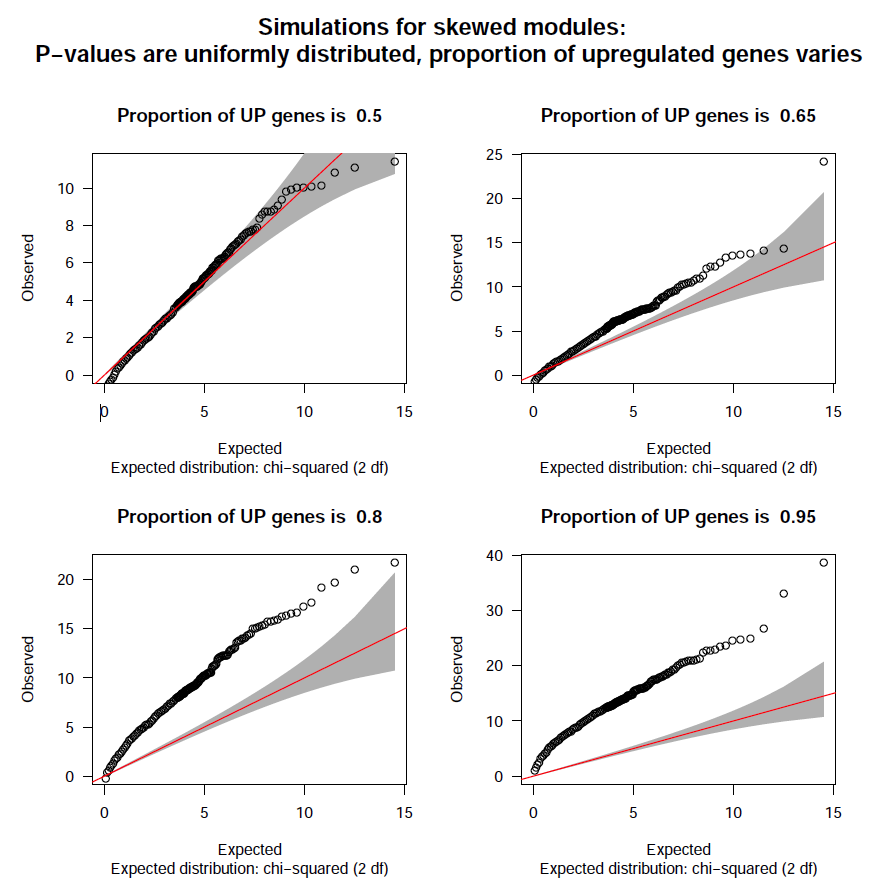
\includegraphics[width=0.8\textwidth]{Figures/Chapter3/simulated_alternative_skewedDir.png}
\caption{\small{Distribution of module-based refined test statistic \textit{p}-values simulated under the alternative plotted against the corresponding expected order chi-squared statistics (two degrees of freedom)} }
    \label{fig:10}
\end{figure}

As can be seen from inspection of Figure 3.4, when the proportion of up-regulated genes is 0.5 our test generates \textit{p}-values highly similar to those seen in the null simulations (Figure 3.3). Naturally the distribution of points is not identical due to random sampling. However, as the module-based proportion of up-regulated genes increases, it can be seen that our \textit{T} results gradually deviate from those expected under a chi-squared with two degrees of freedom. Thus our refined association test successfully enhances the significance of modules containing a high proportion of genes with a common change in expression levels (either up- or down-regulated). The fact that the degree to which the significance is enhanced depends upon the inherent skew in relative proportions of over- and under-expressed genes in a few module dramatically increases the power of this statistical methodology. 

